\documentclass[11pt,letterpaper]{article}

% Essential packages
\usepackage{fontspec}
% \usepackage[utf8]{inputenc}
% \usepackage[T1]{fontenc}
\usepackage{geometry}
\usepackage{amsmath}
\usepackage{amsfonts}
\usepackage{amssymb}
\usepackage{graphicx}
\usepackage{booktabs}
\usepackage{array}
\usepackage{longtable}
\usepackage{multirow}
\usepackage{multicol}
\usepackage{float}
\usepackage{caption}
\usepackage{subcaption}
\usepackage{hyperref}
\usepackage{fancyhdr}
\usepackage{datetime}
\usepackage{enumitem}
\usepackage{listings}
\usepackage{xcolor}
\usepackage{verbatim}
\usepackage{url}
\usepackage{svg}
\usepackage{minted}

% Page setup
\geometry{margin=1in}
\setlength{\parindent}{0pt}
\setlength{\parskip}{6pt}

% handle the bibliography
\bibliographystyle{unsrt}

% Header and footer setup
\pagestyle{fancy}
\fancyhf{}
\lhead{Data Science Capstone: Final Report}
\rhead{\today}
\cfoot{\thepage}
\renewcommand{\headrulewidth}{0.4pt}

% Code listing setup
\lstset{
    basicstyle=\ttfamily\footnotesize,
    backgroundcolor=\color{gray!10},
    frame=single,
    breaklines=true,
    captionpos=b,
    numbers=left,
    numberstyle=\tiny\color{gray},
    keywordstyle=\color{blue},
    commentstyle=\color{green!60!black},
    stringstyle=\color{red}
}

% Custom commands
\newcommand{\workingtitle}{A Statistical Truth Detection System}

\newcommand{\heading}[1]{
    \section*{\workingtitle}
    \addcontentsline{toc}{section}{\workingtitle}
    \textbf{Date:} #1 \\
    \rule{\textwidth}{0.5pt}
}

\newcommand{\motivation}[1]{
    \subsection*{Motivation and Significance}
    \addcontentsline{toc}{subsection}{Motivation and Significance}
    #1
}

\newcommand{\plan}[1]{
    \section*{Project Plan and Timeline}
    \addcontentsline{toc}{section}{Timeline and Milestones}
    #1
}

\newcommand{\data}[2]{
    \section*{Datasets and Models}
    \addcontentsline{toc}{section}{Datasets and Models}
    \subsection*{Datasets}
    #1
    \subsection*{Models}
    #2
}

\newcommand{\problemDefBackground}[1]{
    \section*{Problem Definition and Background}
    \addcontentsline{toc}{section}{Problem Definition and Background}
    #1
}


\newcommand{\methodology}[5]{
    \section*{Methodology}
    \addcontentsline{toc}{section}{Methodology}
    \subsection*{Overview}
    #1
    \subsection*{Models and Algorithms}
    #2
    \subsection*{Tech Stack}
    #3
    \subsection*{Implementation Strategy}
    #4
    \subsection*{Evaluation Metrics}
    #5
}


\newcommand{\eda}[3]{
    \section*{Exploratory Data Analysis}
    \addcontentsline{toc}{section}{Exploratory Data Analysis}
    \subsection*{Data Understanding}
    #1
    \subsection*{Data Cleaning and Preprocessing}
    #2
    \subsection*{Exploratory Data Analysis}
    #3
}

\newcommand{\taskExploration}[3]{
    \section*{Model Tasks Exploration}
    \addcontentsline{toc}{section}{Model Tasks Exploration}
    \subsection*{Task Definition}
    #1
    \subsection*{Feature Engineering}
    #2
    \subsection*{Model Selection}
    #3
}

\newcommand{\baselineModels}[2]{
    \section*{Baseline Models}
    \addcontentsline{toc}{section}{Baseline Models}
    \subsection*{Model Implementation}
    #1
    \subsection*{Model Evaluation}
    #2
}

\newcommand{\createAbstract}[1]{
    \section*{Abstract}
    \addcontentsline{toc}{section}{Abstract}
    #1
}


\newcommand{\intro}[1]{
    \section*{Introduction}
    \addcontentsline{toc}{section}{Introduction}
    #1
}

\newcommand{\litreview}[1]{
    \section*{Literature Review}
    \addcontentsline{toc}{section}{Literature Review}
    #1
}

\newcommand{\design}[3]{
    \section*{Experimental Design}
    \addcontentsline{toc}{section}{Experimental Design}
    \subsection*{Data}
    #1
    \subsection*{Evaluation}
    #2
    \subsection*{Baseline}
    #3
}

\newcommand{\results}[2]{
    \section*{Experimental Results}
    \addcontentsline{toc}{section}{Experimental Results}
    \subsection*{Extensions}
    #1
    \subsection*{Error Analysis}
    #2
}

\newcommand{\conclusion}[1]{
    \section*{Conclusion}
    \addcontentsline{toc}{section}{Conclusion}
    #1
}

\newcommand{\mentor}[5]{
    \subsection*{Mentor Credentials}
    \addcontentsline{toc}{subsection}{Mentor Credentials}
    \begin{itemize}
        \item \textbf{Name:} #1
        \item \textbf{Email:} #2
        \item \textbf{Phone Number:} #3
        \item \textbf{Relevant Skills and Experience:} #4
        \item \textbf{LinkedIn:} #5
    \end{itemize}
}

% Title page setup
\title{\Large \textbf{DATS 598: Data Science Capstone} \\ 
       \large \textbf{DRAFT} Final Report \\
       \vspace{0.5cm}
       \normalsize \textbf{\workingtitle}}
\author{Eric Crisp \\ 
        University of Pennsylvania \\
        \texttt{ecrisp@upenn.edu}}
\date{\today}

\begin{document}

\maketitle
\tableofcontents
\newpage


\createAbstract{

    This project is motivated by the need to have processes in place that reliably determine the validity of information. In this project, various methods such as rule-based and LLM-based methods are used to determine the truthfulness of statements. The intention of this project is to be integrated with a speech-to-text system such as during debates, speeches, or other venues where immediate response to a claim is the desired affect. Other use cases are screening textbooks, news articles, or other forms of information on the internet to help inform the reader. The goal of this project is to make no assumptions as to what is good, or bad, rather focus solely on what is verifiable from a "trusted" source (i.e., Wikipedia). Methods in the literature have been implemented, and extended, to achieve higher than baseline performance on the standard FEVER dataset in classifying whether a claim exists, what the claim is, and classifying it as true, false, or not enough information. This process incorporates a pipeline of methods that are applied to a text string. The pipeline can be configured by the user including thresholds, embedding, and method selections, however, the overall process follows the following architecture: preprocessing, claim detection, claim extraction, query generation, evidence retrieval, and claim verification. A configurable process is to swap the rules-based preprocessing, detection, extraction, and query generation with an API to an LLM (i.e., OpenAI, Claude, or even a fine-tuned BERT). The system is designed to be modular and easily extendable to incorporate new methods as they are developed while maintaining the same performance metrics allowing experimentation and apples-to-apples comparisons.

}

\intro{

    Data science is the process of extracting insights and knowledge from data. Here, the data is considered to be text and the insights are the likelihood of the truthfulness of a claim within that text. Data science is also the science behind scaling these processes such that these automations can be applied reliably and efficiently. In this project, a large amount of effort was put into the scalability of this work. The complex algorithms found in classic computer science problems are absent from this project, but aspects like cleaning, preprocessing, NLP, information retrieval, and machine learning are present to bring a generic string to a verifiable, justifiable conclusion that is a classification of the claims within the string. \\

    This is more than just a simple classification problem, more than just a neural network trained on pattern recognition. This project truly encompasses the data science pipeline. In practice, this project could be applied in real time during debates, speeches, lectures, TedTalks, or any other venue where an audience desires an objective validation on the speakers claims. The goal of this project is to be able to give the average person the ability to be critical of information and rely on the (likelihood of the) truth rather than on opinion alone. A clear example, and perhaps a more applicable example, is scrolling on Instagram, or TikTok, and you see a video raving about the health benefits of of a new diet claiming to be backed by science. Many will take this at face value, but with a fact checking system like this integrated into the platform, having a green checkmark in the corner could turn that 'insightful' video into a misleading hoax just as quickly. Certainly not a flawless system, but for impressionable audiences, this could be a small step in the right direction. \\

    The problem being solved through this project is as follows: given a string of text, determining whether the claims present (if any) are true, false, or not enough information to yield a decision. This is a classification problem, but more-so a problem of information retrieval and information alignment. It is not enough to apply NLP practices, embed, and parse an output. The system must be able to reliably search and retrieve the relevant information, from trusted sources, and determine if the content retrieved confirms, or refutes the claim. This is the problem at hand, and it is not simple due to the nature of dealing with natural language; there are many pitfalls and many (partial) solutions that lead to unintentionally introducing biases, unintended consequences, or are unnecessarily restrictive. These are the problems at hand and will be discussed in detail in the following sections. \\

}

\litreview{

    As mentioned previously, this project is an implementation of an automated fact checking system. The scope, relevance, and applicability has already been established, so the focus of this literature review will be related to the architecture of the system, the methods and processes, as well as the state of the art within the space. \\

    Generally speaking, claims can be classified as true, false, or not enough information (NEI) to classify as true or false. The literature generally describes a pipeline to achieve this classification. The pipeline consists of three main stages: claim detection, evidence retrieval, and claim verification. The first stage is related to distinguishing between what is verifiable and what is not, and how to reliably achieve this. The second stage is related to retrieving evidence directly related to the detected claim from trusted sources. This is where things like document similarity comes into play (TF-IDF, similarity scores, etc.). The third and final stage is the classification. This is where deep learning and ML models can best be applied. \\

    % \cite{automated_fact_check}, \cite{truth_is_universal}, \cite{afc_survey}, \cite{factcheck_editor}, \cite{claimbuster}, \cite{gru}

    Much of the literature relates to the process of handling sentence detection and evidence retrieval.
    White papers, or survey papers, on the field of automated fact-checking consist of generally three
    categories: preprocessing, ranking and evidence retrieval, and multi-classification, or a degree of
    truthfulness. Preprocessing typically consists of two methods, a subject-predicate-object (SPO)
    triplet extraction, or a sentence classification and embedding approach \cite{automated_fact_check, afc_survey}. Ranking and evidence
    retrieval typically consists of a similarity-based approach, a more advanced RAG technique, or
    perhaps more traditionally knowledge graph path traversal ranking \cite{afc_survey, claimbuster}. Document retrieval is one
    of the more challenging parts because of the potentially ambiguous nature of the input. NLP
    techniques require being able to consistently decipher named entities and context understanding
    just to correctly identify the implied, or explicitly stated claim. \\

    The most useful outcome from the literature review is two fold: understanding the processes and
    challenges involved with preprocessing as that appears to be the most consistent hurdle, and consistent reliable databases to pull from rather than requiring a web crawler. Datasets such as FEVER,
    Wikidata, Claimbuster, ClueWeb, Factify are all open source, available databases that can be incorporated into the project for evidence retrieval and truth verification \cite{afc_survey}. The creativity comes with
    how to use the results of retrieval. Some models have done binary classification, others have implemented biased algorithms based on the origination source, others have created knowledge graphs
    for path traversal and ranking to determine the likelihood of truthfulness. \\

    Models used in the literature include ML algorithms in conjunction with NLP techniques such as
    SVM, KNN, random forest, gradient boosting, and Naive Bayes \cite{automated_fact_check, afc_survey, truth_is_universal}. Other references have fine tuned
    LLMs on FEVER and other datasets, such as BERT, neural networks (FNN, RNN, and GRU) \cite{gru}.

}

\design{

    The test data used for evaluation is the FEVER dataset. This consists of 185,445 claims, 145,449 of which are labeled as "SUPPORTS", 19,998 labeled as "REFUTES", and 19,998 labeled as "NOT ENOUGH INFO". Each claim is associated with a set of evidence sentences from Wikipedia that support or refute the claim. Independently, Wikipedia was pulled from an online distribution (English only), and was embedded with a select number of embeddings from Hugging Face. It is worth noting these embeddings do not necessarily reflect the best possible embedding selection, however, were chosen due to simplicity for experimentation and code development. The dataset is designed to evaluate the accuracy, precision, recall, and F1 scores on the processes abilities to determine a claims, extract and embed them, and retrieve relevant evidence to make accurate predictions. \\

    The following are references to the datasets and models used in this project: \\

    \begin{enumerate}
        \item \textbf{FEVER} – A large-scale dataset for fact-checking based on Wikipedia. \\
        \href{https://fever.ai}{https://fever.ai}

        \item \textbf{Wikidata} – A collaboratively edited knowledge base from the Wikimedia Foundation. \\
        \href{https://www.wikidata.org}{https://www.wikidata.org}

        \item \textbf{T5} – A unified framework that casts all NLP tasks as text generation problems. \\
        \href{https://arxiv.org/abs/1910.10683}{https://arxiv.org/abs/1910.10683}

    \end{enumerate}

}{
    
    There are several metrics used to evaluate the performance of the system. The primary metric is accuracy, which measures the proportion of correctly classified claims. Additionally, precision, recall, and F1 score are used to evaluate the performance of the system in more detail. Precision measures the proportion of true positives among all positive predictions, while recall measures the proportion of true positives among all actual positives. The F1 score is the harmonic mean of precision and recall, providing a single metric that balances both. These metrics are calculated for each class (SUPPORTS, REFUTES, NOT ENOUGH INFO) to provide a comprehensive evaluation of the system's performance across different types of claims. It is also important to be able to differentiate between text that contains a claim and text that does not. This is captured by introducing text from the natural language toolkit's Brown library consisting of just text from novels - stories. These are classified as texts without claims. So, on top of evidence retrieval, there are also cases where the system must be able to differentiate without evidence correctly. \\
}{

    From basic testing initially with a rules-based process, the FEVER dataset yielded a claim detection accuracy of 63.4\%, a precision of 80.6\%, and a recall of 35.5\%. This process was barebone and let a lot of claims through when it should not have; hence the high precision, but low recall. This can be seen through the confusion matrix in the figure below.

    \begin{figure}[h!]
        \centering
        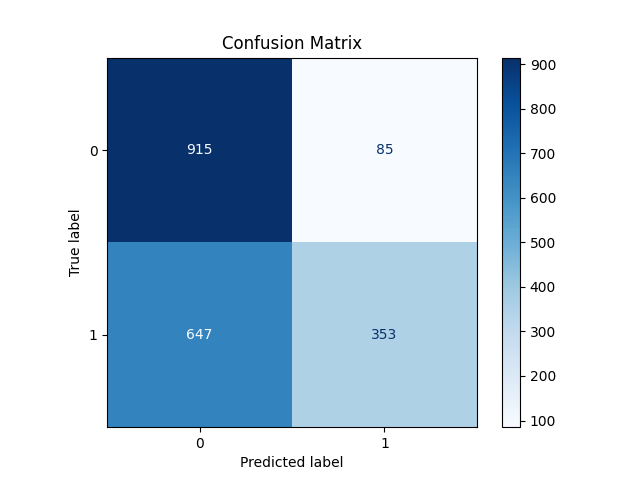
\includegraphics[width=0.8\textwidth]{images/dev_confusion_matrix.png} 
        \caption{Confusion matrix for inital claim detection process.}
        \label{fig:dev_confusion_matrix}
    \end{figure}


}

\results{ 

    Increasing performance is based partially on the increased performance of embedding models whiich were in part selected based on their MTEB ranking \cite{mteb}. A lot of effort was put into making the rules appraoch more balanced. This is exemplified by looking at the figure below, showing a more recent representation of the claim detection process. 

    \begin{figure}[h!]
        \centering
        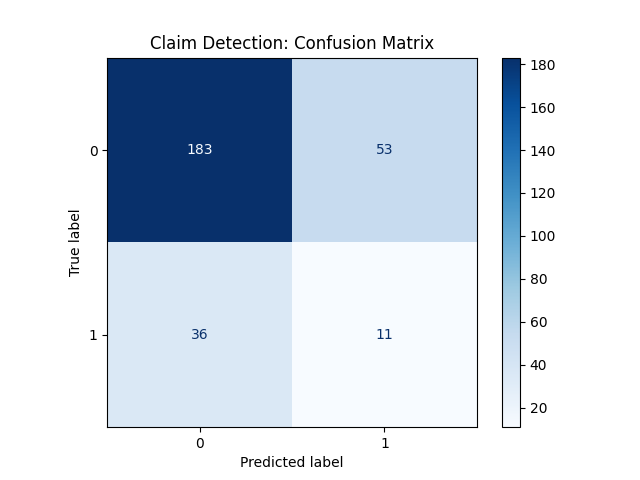
\includegraphics[width=0.8\textwidth]{images/prod_confusion_matrix.png} 
        \caption{Confusion matrix for inital claim detection process.}
        \label{fig:prod_confusion_matrix}
    \end{figure}

}{
    
    The testing harnesses for this system are heavily focused on claim detection and classification. For the error analysis here, it is simple enough to demonstrate the expectation versus the reality of an example. When testing the claim detection process, a block of text is generated with (at random) 0, 1, or 2 claims in a mix of 5 sentences - in any order. This text is then passed into the system and each statement is classified as a claim (e.g., 0) or not a claim (e.g., 1). This forms the basis for the rule-based claim detection. More advanced methods include segmentation of clauses in case a single sentence includes multiple claims and ideally, would include coreference for NER across sentences. However, for a simple example a block of text input to the system could be: \\

    However , it seems axiomatic that the government has an obligation  to exercise its mandate reasonably , equitably and with full regard for the disruptions which it inevitably causes '' . I told him no , that I had had a very happy childhood . And after I brought them sandwiches and coffee I had to go back to my place in the kitchen and wait . The only cardinal sin which may be committed in warming a wine is to force it by putting it next to the stove or in front of an open fire . John McEnroe had rivalries with other tennis players in the 1980's. Phil rubbed his forehead wearily . Rock music originated in the southern United States. \\

    The intended claims include: \\

    John McEnroe had rivalries with other tennis players in the 1980's. \\
    Rock music originated in the southern United States. \\

    As the detection system scans the sentences, applies the procesess and subprocesess, it will generate a Claim object for each claim that is detects as factual and surpasses a threshold. The output of this process would be N objects reflecting the (hopefully) N claims within the text. To determine the metrics, each sentence here would be assigned a 0, or 1, as mentioned earlier depending on if it is known to be a claim. If the system is doing well as detecting claims, these predictions will agree with the labels. This generates the confusion matrix you saw previously. \\

    A very similar process occurs for the higher level classiciation of whether the Claim(s) detected are true, false, or not enough information. The reason for not diving into those results is that the density of the Wikipedia database used is not significant enough to reliably determine the verdict. Given an embedding, if the size of the database does not encompass the content of the embedded query (the claim), then it can artifically yield negative results. \\

}

\conclusion{

    Much of this project relies on series of pipeline processes working together. This project is a toy version of a very scalable, very applicable solution across many audiences. The efforts put forth here illustrate the influence and significance of the various features within the system such as the important of text cleaning and claim detection, the inherent errors associated with rule-based approaches, and the set of thresholds that enable a more dialed in process as a whole. To bring this system up to state of the art, LLM integration for claim detection, claim extraction, and query generation would be optimal. The rules-based approach, although very fast, is error prone. Another implementation that would increase the value of this project is the database used. Only a fraction of Wikipedia was actually used due to computation limitations, however, with the power of the right embedding alongside a comprehensive database (even RAG) this system is capable of generating significant value. \\
}


\bibliography{references}


\end{document}

